% !TEX root = ../main.tex
\chapter{BỘ DỮ LIỆU VÀ THỰC NGHIỆM}
\label{ch:bo_du_lieu_va_thuc_nghiem}

\vspace{-1.5cm} 

\begin{quotation}
    \noindent
    \small\textit{
   Chương này tập trung vào dữ liệu và kết quả thực nghiệm. Nội dung chính gồm đặc điểm của bộ dữ liệu SHOT, hai bộ dữ liệu đánh giá bổ sung BBC Planet Earth và ClipShots, các chỉ số độ chính xác dương, độ bao phủ và F1, sau đó trình bày kết quả định lượng và nhận xét chính trên từng bộ dữ liệu.
    }
\end{quotation}
\vspace{1em} % Tạo khoảng cách nhỏ


\section{Bộ dữ liệu SHOT}
SHOT~\cite{zhu2023autoshot} (Short Video Shot Boundary Detection Dataset) là bộ dữ liệu công khai dành cho tác vụ phát hiện ranh giới cảnh quay (shot boundary detection) trong video ngắn. Các nền tảng video ngắn như TikTok hay Instagram Reels đã thay đổi thói quen tiêu thụ nội dung. Nhu cầu phân tích video chính xác về mặt thời gian là cấp thiết. SHOT cung cấp dữ liệu chuẩn cho video có nhịp độ nhanh và nội dung cô đọng.

Phần lớn các bộ dữ liệu phát hiện biên cảnh (SBD) hiện có như BBC Planet Earth~\cite{baraldi2015rai} chỉ chứa phim tài liệu hoặc talk show với cảnh quay tĩnh và nhịp độ chậm. Ngay cả bộ dữ liệu lớn ClipShots cũng chủ yếu chứa các video dài (trung bình 237 giây). SHOT ra đời để lấp đầy khoảng trống này với tư cách là bộ dữ liệu công khai đầu tiên dành riêng cho video ngắn, bao gồm 853 video hoàn chỉnh và 11.606 chú thích cảnh quay, mang tính thách thức cao hơn về nhịp độ và hiệu ứng hình ảnh.



\subsection{Chi tiết bộ dữ liệu}
\begin{itemize}
    \item \textbf{Tên bộ dữ liệu:} SHOT (Short Video Shot Boundary Detection Dataset)
    \item \textbf{Quy mô:} 853 video ngắn và 11.606 chú thích ranh giới cảnh quay
    \item \textbf{Tổng số khung hình:} 960.794 khung hình
    \item \textbf{Tập kiểm tra:} 200 video với 2.716 chú thích chất lượng cao; chuyên gia kiểm duyệt hai vòng
    \item \textbf{Nguồn dữ liệu:} Video từ một nền tảng video ngắn phổ biến
    \item \textbf{Quyền riêng tư:} Làm mờ khuôn mặt bằng công cụ phát hiện khuôn mặt
    \item \textbf{Phương pháp gán nhãn:} Dùng hình thu nhỏ $48\times27$ cho mỗi khung hình; số thứ tự khung hình hiển thị thích ứng để giảm công sức kiểm tra
    \end{itemize}



\subsection{Phân tích bộ dữ liệu}
SHOT được phân tích dựa trên các thách thức đặc thù của video ngắn:
\begin{itemize}
    \item \textbf{Chuyển cảnh dần phức tạp (Complex Gradual Transitions):} Kết hợp nhiều hiệu ứng chuyển cảnh chồng chéo thay vì cắt cảnh dứt khoát.
    \item \textbf{Cấu trúc tam phân (Ternary Structure):} Video dọc thường giữ nguyên phần trên và dưới (chứa liên kết/thương hiệu), chỉ thay đổi nội dung ở giữa, gây khó khăn cho việc phát hiện.
    \item \textbf{Cảnh ảo (Virtual Scenes):} Các video game với hiệu ứng hình ảnh phóng đại và biến đổi liên tục.
    
\end{itemize}

\begin{figure}[H]
    \centering
    \includegraphics[width=0.8\textwidth]{images/Anh42.png}
    \caption[Minh họa các thách thức đặc thù trong SHOT]{Minh họa các thách thức đặc thù trong SHOT: hàng thứ nhất minh họa chuyển cảnh dần phức tạp, hàng thứ hai minh họa cấu trúc tam phân và hàng thứ ba minh họa cảnh ảo.}
    \label{fig:shot_challenges}
\end{figure}
\FloatBarrier

Sự khác biệt giữa video ngắn và video truyền thống không chỉ nằm ở thời lượng mà còn ở nhịp độ và phong cách hậu kỳ. Bảng~\ref{tab:dataset_comparison_detail} tại Mục~\ref{sec:dataset_summary} trình bày so sánh chi tiết. Các thống kê chính phản ánh tính chất ngắn và nhanh của bộ dữ liệu:
\begin{itemize}
    \item \textbf{Độ dài trung bình video:} 39.5 giây
    \item \textbf{Độ dài trung bình cảnh:} 2.59 giây
    \item \textbf{Phân bố thời lượng:} 90\% video có độ dài dưới một phút
    \item \textbf{Tốc độ chuyển cảnh:} Hầu hết các cảnh trong tập kiểm tra kéo dài dưới 5 giây; video ngắn có nhịp độ sự kiện nhanh hơn video truyền thống
    \end{itemize}

\begin{figure}[H]
    \centering
    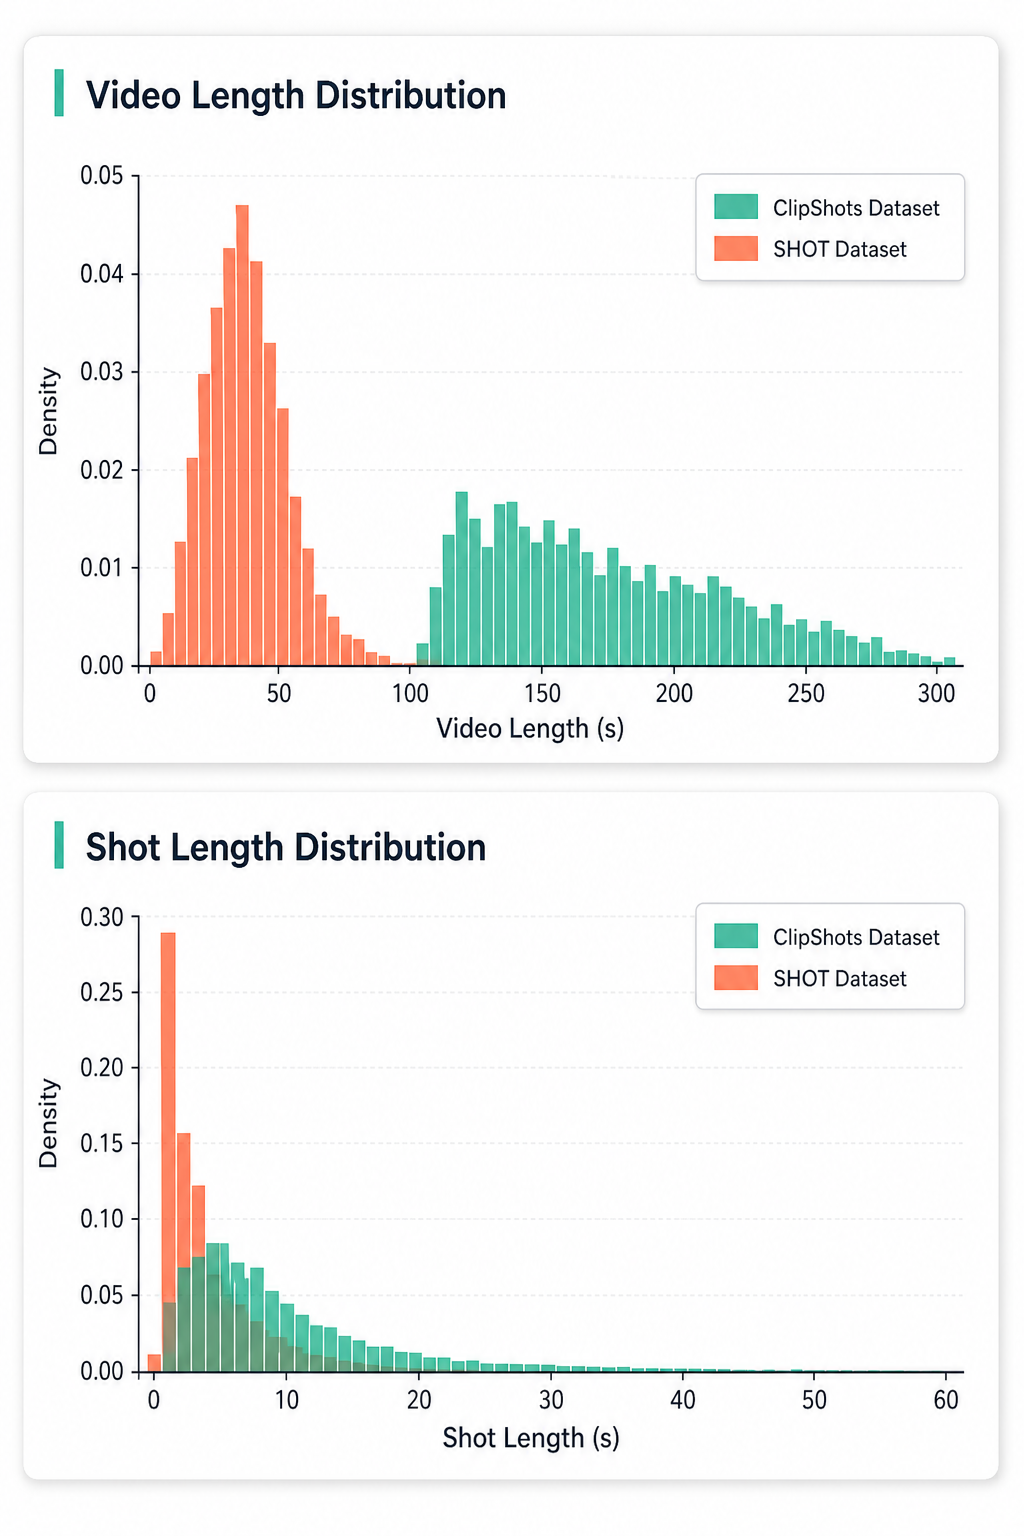
\includegraphics[width=0.5\textwidth]{images/Anh41.png}
    \caption[Phân bố độ dài video và shot trong SHOT]{Sự phân bố độ dài video (trên) và độ dài shot (dưới). Có thể thấy sự chênh lệch rõ rệt: shot trong SHOT tập trung dày đặc ở vùng dưới 5 giây.}
    \label{fig:shot_distribution}
\end{figure}


\subsection{Tóm tắt bộ dữ liệu SHOT}
Trong khóa luận, SHOT là bộ dữ liệu trung tâm để đánh giá hiệu quả trên video ngắn. Các kết quả trên SHOT được dùng để so sánh trực tiếp với TransNetV2, AutoShot gốc và các biến thể AutoShotV2; các kết quả trên BBC và ClipShots được dùng để kiểm tra khả năng tổng quát hóa sang miền dữ liệu khác.
Với các đặc điểm độc đáo phản ánh đúng thực tế của video ngắn và quy trình gán nhãn chất lượng cao, SHOT không chỉ là một chuẩn mực đánh giá mới mà còn là một tài nguyên quý giá để huấn luyện các mô hình SBD thế hệ tiếp theo. Các kết quả thực nghiệm chi tiết trên SHOT và các bộ dữ liệu bổ sung được trình bày ở các mục kết quả phía sau.

\section{Các bộ dữ liệu đánh giá bổ sung}
Ngoài bộ dữ liệu SHOT dành riêng cho video ngắn, các nghiên cứu về phát hiện ranh giới cảnh quay thường được đánh giá trên nhiều bộ dữ liệu chuẩn khác nhau để kiểm tra khả năng tổng quát hóa. Phần này giới thiệu chi tiết hai bộ dữ liệu phổ biến: BBC Planet Earth và ClipShots. Những bộ dữ liệu này đại diện cho các miền nội dung và thách thức khác nhau, giúp đánh giá toàn diện hiệu năng của các mô hình SBD.

\subsection{Bộ dữ liệu BBC Planet Earth}
\textbf{BBC Planet Earth}~\cite{baraldi2015rai} gồm 11 tập phim tài liệu thiên nhiên. Mỗi tập dài khoảng 50 phút; toàn bộ dữ liệu có khoảng 4.900 cảnh quay, với độ dài cảnh quay trung bình 6,57 giây. Nội dung chất lượng cao với các chuyển động lia và thu phóng máy quay mượt mà và phong cách biên tập nghệ thuật sử dụng nhiều hiệu ứng chồng hình và mờ dần. Thách thức chính là \textbf{chuyển cảnh dần} phức tạp khiến ranh giới giữa hai shot không sắc nét như chuyển cảnh đột ngột.

\subsection{Bộ dữ liệu ClipShots}
\textbf{ClipShots}~\cite{tang2018clipshots} là bộ dữ liệu quy mô lớn từ YouTube và Weibo, gồm 4.039 video với độ dài trung bình 237 giây, hơn 128.000 chuyển cảnh đột ngột và hơn 38.000 chuyển cảnh dần được dán nhãn thủ công. Độ dài cảnh quay trung bình là 15,34 giây và nội dung trải rộng trên hơn 20 danh mục từ nghiệp dư đến chuyên nghiệp. Thách thức: thay đổi ánh sáng đột ngột, camera rung, hiệu ứng chuyển cảnh không quy ước, chẳng hạn nhiễu hình, lóe sáng và thu phóng nhanh, cùng khoảng cách miền dữ liệu lớn.

\subsection{So sánh tổng hợp các bộ dữ liệu}
\label{sec:dataset_summary}
Bảng \ref{tab:dataset_comparison_detail} tổng hợp các đặc điểm chính của ba bộ dữ liệu được sử dụng trong đánh giá hiệu năng các mô hình SBD.

\begin{table}[H]
\centering
\small
\begin{tabularx}{\textwidth}{l Y Y Y}
\toprule
\textbf{Đặc điểm} & \textbf{BBC} & \textbf{ClipShots} & \textbf{SHOT} \\
\midrule
Loại nội dung & Phim tài liệu & Đa dạng & Video ngắn \\
Số lượng video & 11 & 4{,}039 & 853 \\
Độ dài TB video (s) & 2{,}945 & 237 & 39.5 \\
Độ dài TB shot (s) & 6.57 & 15.34 & 2.59 \\
Chuyển cảnh đột ngột & Nhiều & 128{,}000+ & 8{,}890 \\
Chuyển cảnh dần & Rất nhiều & 38{,}000+ & 2{,}716 \\
Độ khó & Trung bình & Cao & Rất cao \\
Thách thức chính & Chuyển cảnh dần & Đa dạng hiệu ứng & Nhịp độ nhanh \\
\bottomrule
\end{tabularx}
\caption{So sánh chi tiết các bộ dữ liệu đánh giá SBD}
\label{tab:dataset_comparison_detail}
\end{table}

Mỗi bộ dữ liệu đại diện cho một khía cạnh khác nhau của bài toán SBD trong thực tế:
\begin{itemize}
    \item \textbf{BBC Planet Earth:} Đánh giá khả năng xử lý chuyển cảnh dần dần trong nội dung chuyên nghiệp.
    \item \textbf{ClipShots:} Đánh giá khả năng tổng quát hóa trên nội dung thế giới mở đa dạng.
    \item \textbf{SHOT:} Đánh giá hiệu năng trên video ngắn với nhịp độ nhanh và hiệu ứng phức tạp.
\end{itemize}

\section{Các chỉ số đánh giá hiệu quả mô hình}
\label{sec:metrics}

Do dữ liệu SBD mất cân bằng nghiêm trọng (khung hình không chuyển cảnh chiếm đa số), khóa luận dùng bộ ba chỉ số độ chính xác dương (Precision), độ bao phủ (Recall) và chỉ số F1 thay cho độ chính xác tổng thể (Accuracy). Ký hiệu: $N_c$ (TP), $N_m$ (FN), $N_f$ (FP) lần lượt là số ranh giới phát hiện đúng, bỏ sót, và báo động giả. Ngưỡng $\theta$ chuyển xác suất đầu ra thành quyết định nhị phân: dự đoán $> \theta$ được coi là ranh giới.

\begin{align}
    \text{Precision} &= \frac{N_c}{N_c + N_f}, \\
    \text{Recall} &= \frac{N_c}{N_c + N_m}, \\
    \text{F1} &= 2 \times \frac{\text{Precision} \times \text{Recall}}{\text{Precision} + \text{Recall}}.
\end{align}

Độ chính xác dương cao đồng nghĩa ít báo động giả; độ bao phủ cao đồng nghĩa ít bỏ sót ranh giới. F1 là trung bình điều hòa của hai chỉ số, được dùng làm tiêu chí so sánh chính giữa các phương pháp vì nó phản ánh đồng thời cả hai chiều. Việc đánh giá trên nhiều bộ dữ liệu (SHOT, ClipShots, BBC) là cần thiết để kiểm tra khả năng tổng quát hóa.

\section{Kịch bản thực nghiệm}
\label{sec:experimental_scenarios}
Các kết quả trong khóa luận được tổ chức theo ba nhóm: kết quả chính (F1 tốt nhất theo từng bộ dữ liệu, đúng giao thức đánh giá của AutoShot), so sánh độ chính xác dương, độ bao phủ và F1, và các bảng kết quả bổ sung để giải thích xu hướng quan sát được. Phần thảo luận về lỗi và khả năng tổng quát hóa được chuyển sang Chương~\ref{ch:ket_luan}.

Để bảo đảm khả năng tái lập, toàn bộ thí nghiệm được chạy với hạt giống ngẫu nhiên cố định 42. Các kết quả thực nghiệm phân rã sử dụng cùng cách phân chia huấn luyện/xác thực/kiểm tra, cùng tệp trọng số AutoShot gốc và cùng siêu dữ liệu. Những tệp nặng như tệp trọng số, logit đã lưu đệm và bộ dữ liệu video không được đưa vào Git, mà được quản lý riêng theo bản kê tệp (manifest). Chi tiết về môi trường phần cứng và phiên bản thư viện được mô tả cụ thể trong Bảng~\ref{tab:execution_environment}.

\begin{table}[H]
\centering
\small
\caption{Môi trường thực thi và cấu hình thực nghiệm}
\label{tab:execution_environment}
\begin{tabularx}{\textwidth}{lX}
\toprule
\textbf{Hạng mục} & \textbf{Giá trị} \\
\midrule
Hệ điều hành & Windows 10 Pro 19045 (local) và Kaggle Linux tùy theo lượt chạy \\
Python & 3.12.7 (Anaconda) \\
PyTorch & 2.5.1 (build cu121) \\
CUDA & 12.1 (nếu dùng GPU build) \\
GPU & Kaggle P100/T4 cho huấn luyện \\
Thư viện chính & numpy 2.2.6, scipy 1.17.1, einops 0.8.2, opencv-python 4.12.0.88, pillow 10.4.0, matplotlib 3.10.8 \\
Hạt giống (Seed) & 42 \\
\bottomrule
\end{tabularx}
\end{table}

\subsection{Cấu hình cuối cùng của AutoShotV2}
Khóa luận báo cáo kết quả của AutoShotV2 ở \textbf{ngưỡng cho F1 cao nhất trên từng bộ dữ liệu}, đúng theo giao thức đánh giá chuẩn của AutoShot gốc. Giao thức này quét một dải ngưỡng quyết định rồi chọn F1 cao nhất cho mỗi bộ dữ liệu, như trình bày tại Mục~\ref{sec:extra_param_sweep}. Nhờ dùng chung giao thức chọn ngưỡng với AutoShot, kết quả của hai mô hình được so sánh trực tiếp và công bằng.

Hệ thống gồm các thành phần:
\begin{itemize}
    \item \textbf{Mạng xương sống:} Kiến trúc AutoShot@F1 (đã được NAS tối ưu và đóng băng trọng số).
    \item \textbf{Tầng phân loại:} Bộ phân lớp mới huấn luyện lại từ đặc trưng đã lưu đệm với hàm mất mát Focal ($\gamma=2.0$, $\alpha=0.6$) và nhãn nhiều điểm dương với trọng số 0,3.
    \item \textbf{Hậu xử lý:} Hiệu chỉnh nhiệt độ, làm mượt Gaussian với $\sigma=2.0$, và ngưỡng quyết định chọn theo từng bộ dữ liệu.
\end{itemize}

Cả ba bộ dữ liệu dùng \textbf{chung một cấu hình duy nhất}: hệ số nhiệt độ $T^* = 0.2413$, $\sigma = 2.0$, Focal Loss $\gamma = 2.0$, $\alpha = 0.6$, trọng số nhánh nhiều điểm dương $0.3$, tốc độ học $7\times10^{-6}$ và suy giảm trọng số $10^{-4}$. Phụ lục~\ref{sec:hparam_search} trình bày chi tiết quá trình tìm kiếm siêu tham số. Các bộ dữ liệu chỉ khác nhau ở ngưỡng quyết định được chọn riêng theo Bảng~\ref{tab:autoshotv2_dataset_thresholds}.

\begin{table}[H]
\centering
\small
\caption{Ngưỡng quyết định của cấu hình chính theo từng bộ dữ liệu}
\label{tab:autoshotv2_dataset_thresholds}
\begin{tabular}{lc}
\toprule
\textbf{Bộ dữ liệu} & \textbf{Ngưỡng quyết định} \\
\midrule
SHOT & 0.12 \\
ClipShots & 0.19 \\
BBC & 0.12 \\
\bottomrule
\end{tabular}
\end{table}

\section{Kết quả chính trên SHOT và các bộ dữ liệu bổ sung}
\label{sec:main_results}

Bảng~\ref{tab:autoshotv2_results} tổng hợp F1-score của toàn bộ các phiên bản đã thực hiện trong khóa luận cùng các mô hình tham chiếu (TransNetV2, AutoShot gốc và một số công trình kinh điển) trên ba bộ dữ liệu SHOT, BBC và ClipShots, nhằm kiểm chứng các giả thuyết nghiên cứu RQ1 và RQ3. Cấu hình chính của AutoShotV2 được báo cáo ở \textbf{ngưỡng cho F1 cao nhất trên từng bộ dữ liệu} --- đúng theo giao thức đánh giá của AutoShot gốc (quét một dải ngưỡng quyết định rồi chọn F1 cao nhất cho mỗi bộ dữ liệu), nhờ vậy con số của AutoShotV2 và AutoShot được so sánh trên cùng một quy trình. Bên cạnh đó, nhóm còn báo cáo một số biến thể khác nhau ở \textit{tập dữ liệu dùng huấn luyện lại tầng phân loại} (Pha 2): chỉ SHOT, chỉ ClipShots, và chỉ ClipShots kèm trung bình trượt lũy thừa trọng số (EMA), nhằm cho thấy không phiên bản nào thắng tuyệt đối trên cả ba miền. Ô ``--'' là cấu hình chưa được đánh giá trên tập tương ứng.

\begin{table}[H]
\centering
\small
\setlength{\tabcolsep}{5pt}
\renewcommand{\arraystretch}{1.2}
\caption[So sánh F1-score các phiên bản trên SHOT, BBC và ClipShots]{So sánh F1-score của toàn bộ các phiên bản và mô hình tham chiếu trên SHOT, BBC và ClipShots. AutoShotV2 (cấu hình chính) và AutoShotV2-HeatMap đều báo cáo ở ngưỡng cho F1 cao nhất trên mỗi tập, đúng theo giao thức đánh giá của AutoShot gốc. Ô ``--'' là cấu hình chưa được đánh giá trên tập tương ứng.}
\label{tab:autoshotv2_results}
\begin{tabular}{L{4.4cm}L{4.0cm}C{1.35cm}C{1.35cm}C{1.5cm}}
\toprule
\textbf{Phương pháp} & \textbf{Mô tả} & \textbf{SHOT} & \textbf{BBC} & \textbf{ClipShots} \\
\midrule
Deep Structured Models & Công trình kinh điển (theo báo cáo) & -- & 0.8920 & 0.7030 \\
TransNet V1 & Công trình kinh điển (theo báo cáo) & -- & 0.9290 & 0.7350 \\
TransNetV2 & Mô hình cơ sở thủ công (theo báo cáo) & 0.7993 & 0.9620 & 0.7760 \\
AutoShot (báo cáo gốc) & AutoShot gốc, số công bố & 0.8410 & 0.9710 & 0.7870 \\
AutoShot (tự chạy lại) & AutoShot gốc, tái lập trong khóa luận & 0.8405 & 0.9554 & 0.7649 \\
\midrule
AutoShotV1 & AutoShot@F1 + Gaussian, không huấn luyện lại & 0.8477 & -- & -- \\
\textbf{AutoShotV2 (cấu hình chính)} & Huấn luyện lại tầng phân loại; ngưỡng tốt nhất theo từng bộ & \textbf{0.8607} & \textbf{0.9648} & 0.7706 \\
AutoShotV2 (chỉ Shot) & Huấn luyện lại tầng phân loại chỉ trên SHOT & 0.8552 & 0.9512 & 0.7241 \\
AutoShotV2 (chỉ ClipShots) & Huấn luyện lại tầng phân loại chỉ trên ClipShots & 0.8371 & 0.9494 & 0.7638 \\
AutoShotV2 (chỉ ClipShots + EMA) & Như trên, thêm trung bình trượt EMA trọng số & 0.8417 & 0.9604 & \textbf{0.7860} \\
AutoShotV2-HeatMap & + nhãn mềm dạng heatmap (thiên Recall) & 0.8557 & -- & 0.7560 \\
\bottomrule
\end{tabular}
\end{table}

\textbf{Nhận xét:} Bảng~\ref{tab:autoshotv2_results} cho thấy các kiến trúc thế hệ sau (từ TransNetV2 trở đi) vượt trội rõ rệt so với các công trình kinh điển (DSM, TransNet V1). Trong nhóm AutoShotV2, \textbf{cấu hình chính đạt F1 cao nhất trên SHOT ($0.8607$)} --- vượt AutoShot gốc tự chạy lại ($0.8405$, tức $+2.0$ điểm phần trăm) và cả các biến thể khác (HeatMap $0.8557$, only-Shot $0.8552$); trên ClipShots biến thể huấn luyện trên ClipShots kèm EMA đạt cao nhất ($0.7860$) trong khi biến thể chỉ dùng SHOT tụt còn $0.7241$ --- khẳng định ClipShots nhạy với dữ liệu và cấu hình theo miền; trên BBC khoảng cách giữa các phiên bản nhỏ ($0.949$--$0.966$). Vì mục tiêu đề tài là video ngắn, cấu hình chính được lựa chọn theo hiệu năng cao nhất trên SHOT, đồng thời vẫn giữ khả năng tổng quát hóa tốt trên BBC và ClipShots; chi tiết ngưỡng quyết định theo từng bộ được trình bày ở Mục~\ref{sec:extra_param_sweep}. Hai phiên bản phụ trợ AutoShotV1 (chỉ bổ sung làm mượt Gaussian) và AutoShotV2-HeatMap (nhãn mềm dạng heatmap) chỉ được đưa vào bảng để so sánh; phần mô tả và phân tích chi tiết của chúng được trình bày ở Phụ lục~\ref{sec:variants_v1_heatmap}.

\section{Kết quả chính: Precision, Recall, F1 theo từng bộ dữ liệu}
\label{sec:extra_param_sweep}

\textbf{Mục đích thí nghiệm:} Mục này báo cáo kết quả chính của AutoShotV2 --- Precision, Recall và F1 tại \textbf{ngưỡng cho F1 cao nhất trên từng bộ dữ liệu}, đúng theo giao thức đánh giá của AutoShot gốc\footnote{Tương ứng hàm đánh giá \texttt{mAP\_f1\_p\_fix\_r} trong mã nguồn AutoShot gốc: quét một dải ngưỡng quyết định rồi lấy F1 cao nhất cho mỗi bộ dữ liệu.}. Nhờ dùng chung giao thức, con số của AutoShotV2 và AutoShot được so sánh trực tiếp và công bằng.

Cấu hình chính dùng bộ siêu tham số: $T^*=0.2413$, $\sigma=2.0$, $\gamma=2.0$, $\alpha=0.6$, trọng số nhãn nhiều điểm dương bằng $0.3$, tốc độ học bằng $7\times10^{-6}$ và suy giảm trọng số bằng $10^{-4}$ (chi tiết quá trình tìm kiếm siêu tham số ở Phụ lục~\ref{sec:hparam_search}). Cùng một cấu hình này được dùng cho cả ba bộ dữ liệu, chỉ khác ngưỡng quyết định chọn riêng cho từng bộ: SHOT tại $\theta=0.12$, ClipShots tại $\theta=0.19$ và BBC tại $\theta=0.10$.

\begin{table}[H]
\centering
\caption[Precision, Recall, F1 của AutoShotV2 theo từng bộ dữ liệu]{Precision, Recall, F1 của AutoShotV2 (cấu hình chính) ở ngưỡng cho F1 cao nhất trên mỗi bộ dữ liệu. Cột cuối là mức cải thiện F1 so với AutoShot tự chạy lại (SHOT $0.8405$, ClipShots $0.7649$, BBC $0.9554$).}
\label{tab:extra_sweep_peaks}
\small
\setlength{\tabcolsep}{3pt}
\begin{tabular}{L{3.0cm}C{1.8cm}C{2.0cm}C{1.8cm}C{1.5cm}C{2.4cm}}
\toprule
\textbf{Bộ dữ liệu} & \textbf{Ngưỡng} & \textbf{Precision} & \textbf{Recall} & \textbf{F1} & \textbf{$\Delta$F1 vs AutoShot (điểm \%)} \\
\midrule
SHOT & 0.12 & 0.8408 & 0.8816 & \textbf{0.8607} & $+2.02\%$ \\
ClipShots & 0.19 & 0.7011 & 0.8554 & \textbf{0.7706} & $+0.57\%$ \\
BBC & 0.12 & 0.9668 & 0.9628 & \textbf{0.9648} & $+0.94\%$ \\
\bottomrule
\end{tabular}
\end{table}

\textbf{Kết quả minh chứng:} Các giá trị Precision/Recall/F1 và ngưỡng tương ứng được ghi nhận chi tiết tại Bảng~\ref{tab:extra_sweep_peaks}.

\textbf{Thảo luận:} Trên SHOT --- bộ dữ liệu trọng tâm của đề tài --- AutoShotV2 đạt F1 $0.8607$, cao hơn AutoShot tự chạy lại $+2.0$ điểm phần trăm dưới cùng một giao thức chọn ngưỡng. Trên BBC, mô hình tổng quát hóa tốt ($0.9648$, cao hơn AutoShot $0.9554$ và TransNetV2 tự chạy lại $0.9593$). Trên ClipShots, F1 đạt $0.7706$ với Recall cao ($0.8554$) nhưng Precision thấp hơn hẳn ($0.7011$): mô hình bắt được phần lớn ranh giới thật nhưng vẫn sinh nhiều dự đoán dư thừa trên phân phối video thế giới mở đa dạng --- đây là hạn chế chính còn tồn tại trên miền dữ liệu này. Lưu ý ngưỡng $0.12$ và $0.19$ được lấy trên lưới mịn hơn dải ngưỡng mặc định của AutoShot, và được áp dụng đồng nhất cho cả AutoShotV2 lẫn các mô hình tham chiếu để bảo đảm so sánh công bằng.

\section{Thực nghiệm phân rã thành phần}
\label{sec:ablation}

\textbf{Mục đích thí nghiệm:} Thực nghiệm phân rã thành phần (ablation study) này nhằm kiểm chứng độc lập và làm rõ đóng góp thực tế của từng đề xuất cải tiến (gồm hàm mất mát Focal, nhãn nhiều điểm dương ở giai đoạn huấn luyện; hiệu chỉnh nhiệt độ - temperature scaling, làm mượt Gaussian - Gaussian smoothing ở giai đoạn hậu xử lý) trên quy trình (pipeline) Pha 2 (đóng băng mạng xương sống) đối với hiệu năng cuối cùng của hệ thống, trả lời cho câu hỏi nghiên cứu RQ2.

Bảng~\ref{tab:ablation_controlled} phân tách đóng góp của từng thành phần trên quy trình Pha 2 --- chỉ huấn luyện lại tầng phân loại trên đặc trưng đã trích sẵn (đóng băng mạng xương sống) --- theo một ma trận đối chứng có kiểm soát. Lưu ý ma trận này chạy trên tập con metadata (dùng cho kiểm định chéo) với hệ số nhiệt độ riêng, nên F1 tuyệt đối không so trực tiếp được với kết quả chính ở Mục~\ref{sec:extra_param_sweep}; bảng chỉ nhằm đọc mức chênh $\Delta$F1 giữa các cấu hình thành phần.

\begin{table}[H]
\centering
\caption[Ablation thành phần có kiểm soát trên Pha 2]{Ablation thành phần có kiểm soát trên Pha 2: $\Delta$F1 so với đối chứng A1 (điểm phần trăm). Số đậm đánh dấu cấu hình $B4$ được chọn làm cấu hình hậu xử lý chính.}
\label{tab:ablation_controlled}
\small
\begin{tabular}{L{5.0cm}C{2.2cm}C{2.2cm}C{2.4cm}}
\toprule
\textbf{Cấu hình} & \textbf{SHOT} & \textbf{BBC} & \textbf{ClipShots} \\
\midrule
\AblationRows
\bottomrule
\end{tabular}
\end{table}

\textbf{Kết quả minh chứng:} Ma trận kết quả ablation có kiểm soát được chi tiết hóa tại Bảng~\ref{tab:ablation_controlled}.

\textbf{Thảo luận:} Trong ma trận đối chứng có kiểm soát ở Bảng~\ref{tab:ablation_controlled}, quá trình ablation được thực hiện trên quy trình Pha 2 bằng cách huấn luyện tầng phân loại trên đặc trưng đã trích sẵn (đóng băng mạng xương sống). Cấu hình đối chứng (control) là $A1$ (huấn luyện với hàm BCE và nhãn một điểm dương (one-hot)). Quá trình hậu xử lý trong thí nghiệm này sử dụng hệ số nhiệt độ $T^*=0.6618$ (khác hệ số nhiệt độ của cấu hình chính do chạy trên tập con metadata dùng cho cross-validation). Mô hình AutoShot gốc $A0$ đóng vai trò mốc tham chiếu. Số đậm trong bảng đánh dấu cấu hình $B4$ được chọn làm cấu hình hậu xử lý chính trong ma trận đối chứng chứ không phải giá trị lớn nhất của cột.

Trong ma trận đối chứng này, hậu xử lý là đòn bẩy lớn nhất: $B4$ (Hiệu chỉnh nhiệt độ + Làm mượt Gaussian) nâng F1 rõ rệt so với đối chứng $A1$ trên SHOT ($+1.6$ điểm phần trăm) và ClipShots ($+4.6$ điểm phần trăm), trong khi hàm mất mát Focal hay nhãn nhiều điểm dương riêng lẻ gần như không thay đổi. Cấu hình $P1$ (chỉ làm mượt Gaussian) tuy tăng mạnh ClipShots nhưng làm giảm BBC xuống dưới ngưỡng guardrail, nên không được chọn; B4 giữ BBC gần như không đổi, cung cấp bằng chứng thực nghiệm rằng hiệu chỉnh nhiệt độ kết hợp làm mượt Gaussian là hướng hậu xử lý ổn định nhất trong thí nghiệm đối chứng.

Nhận xét từ bảng phân rã thành phần:
\begin{itemize}
    \item \textbf{Hậu xử lý là thành phần tác động lớn nhất:} Làm mượt Gaussian, đặc biệt khi kết hợp với hiệu chỉnh nhiệt độ ở $B4$, cải thiện rõ rệt trên ClipShots và SHOT; các thành phần huấn luyện như hàm mất mát Focal hay nhãn nhiều điểm dương chỉ tạo thay đổi nhỏ hoặc không ổn định khi đứng độc lập.
    \item \textbf{ClipShots vẫn là miền thử thách cực lớn:} Việc tinh chỉnh tầng phân loại chưa thể giúp mô hình vượt qua baseline gốc một cách ổn định trên ClipShots ở các cấu hình đối chứng, củng cố nhận định rằng miền dữ liệu thế giới mở này cần các cơ chế hiệu chỉnh nhiệt độ hoặc làm mượt thích nghi miền riêng biệt.
\end{itemize}

\begin{figure}[H]
\centering
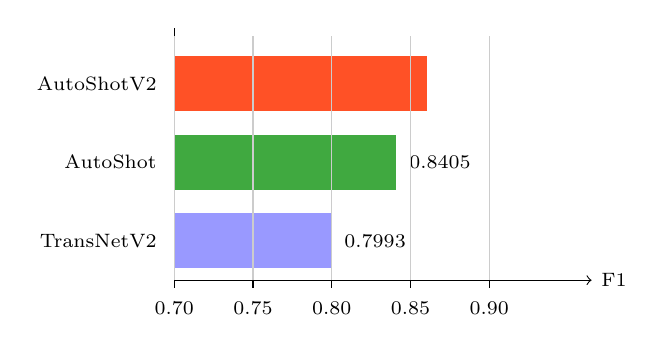
\begin{tikzpicture}[font=\small]
% Horizontal bar chart comparing F1 scores
% Scale: display_x = (value - 0.70) * 20
% [0.70, 0.95] → [0, 5] cm

% Bar heights (y centers) and half-height
\def\yA{2.4}  % AutoShotV2
\def\yB{1.4}  % AutoShot
\def\yC{0.4}  % TransNetV2
\def\hh{0.35}

% Bars
% TransNetV2 F1=0.7993 → (0.7993-0.7)*20=1.986
\fill[blue!50, opacity=0.8]        (0,\yC-\hh) rectangle (1.986,\yC+\hh);
% AutoShot F1=0.8405 → 2.810
\fill[green!55!black, opacity=0.75](0,\yB-\hh) rectangle (2.810,\yB+\hh);
% AutoShotV2 best F1=0.8607 -> 3.214
\fill[red!60!orange, opacity=0.85] (0,\yA-\hh) rectangle (3.214,\yA+\hh);

% Value labels
\node[anchor=west, font=\scriptsize]        at (2.036, \yC) {0.7993};
\node[anchor=west, font=\scriptsize]        at (2.860, \yB) {0.8405};
\node[anchor=west, font=\scriptsize\bfseries] at (3.264, \yA) {\textbf{\ASVTwoBestShotFOne{}}};

% Model name labels
\node[anchor=east, font=\scriptsize] at (-0.1, \yC) {TransNetV2};
\node[anchor=east, font=\scriptsize] at (-0.1, \yB) {AutoShot};
\node[anchor=east, font=\scriptsize] at (-0.1, \yA) {AutoShotV2};

% X-axis and ticks
\draw[->] (0,-0.1) -- (5.3,-0.1) node[right, font=\scriptsize] {F1};
\draw     (0,-0.1) -- (0,3.1);
\foreach \v/\x in {0.70/0, 0.75/1, 0.80/2, 0.85/3, 0.90/4} {
  \draw[gray!40, thin] (\x, -0.1) -- (\x, 3.0);
  \draw (\x,-0.1) -- (\x,-0.2);
  \node[below, font=\scriptsize] at (\x,-0.25) {\v};
}
\end{tikzpicture}
\caption[So sánh F1 trên tập SHOT]{So sánh F1 giữa các mô hình trên tập SHOT (200 video kiểm tra). AutoShotV2 đạt F1 = \ASVTwoBestShotFOne{} theo lựa chọn tốt nhất trong protocol so sánh chính, cải thiện $+\ASVTwoBestVsAutoShotShotPP{}$ điểm phần trăm so với AutoShot tự chạy lại và $+\ASVTwoBestVsTransNetShotPP{}$ điểm phần trăm so với TransNetV2 mô hình cơ sở.}
\label{fig:f1_comparison}
\end{figure}
\FloatBarrier





\section{Tổng kết chương}
Chương này đã trình bày các bộ dữ liệu được sử dụng, đặc điểm chính của SHOT và hai bộ dữ liệu đánh giá bổ sung BBC, ClipShots, cùng bộ chỉ số độ chính xác dương, độ bao phủ và F1. Trên cơ sở đó, chương báo cáo kết quả đánh giá AutoShotV2 trên từng bộ dữ liệu, so sánh với các mô hình tham chiếu và phân tích xu hướng độ chính xác dương, độ bao phủ và F1. Những nội dung thảo luận sâu về lỗi còn tồn tại và khả năng tổng quát hóa được đặt ở Chương~\ref{ch:ket_luan}.
